\chapter{Vehicular Ad-hoc Networks}
\label{chap:vanets}

The prospect of autonomous vehicles makes the study of Vehicular Ad-hoc Networks (VANETs) important.
However, it will still take many years before completely autonomous vehicles are the norm and, until then, VANETs can be a valuable tool to help drivers reduce travel times and diminish the risk of collisions.
Thousands of people die each year due to traffic accidents, many of which could have been avoided if vehicles were smarter and able to provide important alerts both to their drivers and to neighboring vehicles.
The vehicles' on-board computers can aid drivers to increase safety and reduce traffic, but data needs to be shared among the various vehicles in the network.
Such data includes location, speed and destination, which neighboring vehicles can use to adjust their trajectory and increase their own efficiency.
% By allowing vehicles to share their locations, speeds, and destinations with each other, traffic can become more stable and predictable.

\begin{figure}[h]
    \centering
    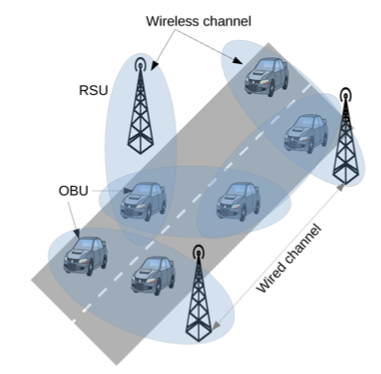
\includegraphics[width=0.5\textwidth]{images/vanet.png}
    \caption{Basic elements of a VANET: OBUs and RSUs. \cite{saini2015close}}
    \label{fig:vanet}
\end{figure}

Current efforts to make VANETs viable in cities are centered around the IEEE 802.11p standard, also called Wireless Access in Vehicular Environments (WAVE) \cite{jiang2008ieee}.
Amongst other aspects of the wireless technology, the WAVE standard describes two types of nodes for vehicular networks: on-board units (OBUs) and road-side units (RSUs).
On-board units are computers placed within each vehicle which monitor the vehicle's data and are able to communicate with other nodes using wireless signals.
Road-side units are placed in static locations near roads; they may also have wired interfaces with other RSUs and the Internet, so it is possible to use them as anchor points for Internet access for passing vehicles.

%[description of trust in context of VANETs]

\section{Trust in VANETs}

Like in other types of networks, the proper functioning of a VANET depends on the reliability of the vehicles (nodes) of the network.
If one node is malicious or faulty, it can spread incorrect data that may compromise the utility of the VANET.
Once the concept of VANETs was established, researchers have been attempting to predict ways in which malicious users might use the network to their advantage.
Examples include triggering false alarms about inexistent accidents, lying about the average speed in one road to make it less desirable for others, and falsifying geolocation data to exploit location-based routing algorithms. Therefore, the concept of trust must be established in the vehicular network context, allowing for nodes to judge the validity of information transmitted by others and share those conclusions with other nodes.

There is an important distinction between a malicious node and a faulty one; both of them may be sharing false data, but for different reasons and with different consequences.
For example, a malicious node may lie about its location in order to make routing protocols use it \cite{leinmuller2005influence}, in order to try to store or alter messages, while a faulty GPS module may cause an accident because its position data was incorrect.
However, that distinction can be hard to make, because a close inspection is necessary to determine whether the incorrect data is erratic or deliberate.
Since both types of nodes are problematic to the proper functioning of a network, malicious and faulty nodes can be treated as the same in a trust model.

%\textbf{/*********}
%Trust can be a related, yet distinct, issue to cryptography and authentication in vehicular networks.
%Many studies propose the use of a PKI (Public Key Infrastructure) to guarantee legitimate identities for nodes, although this solution requires, by definition, a certifying authority to manage and distribute public keys.
%VANETs must be able to function in a completely independent fashion, regardless of the amount of active nodes in a given region, and without relying on a centralized service.
%Both trust and authentication must work together to provide an adequate solution for VANETs, since it is difficult to establish trust without means to verify an identity (a malicious node may provide false data about its identity to bypass trust solutions), while a cryptography system requires a pre-existing infrastructure and may add unacceptable latency to high-priority messages.
%\textbf{[moved to chapter 4]}
%\textbf{*********/}

In general, trust management solutions for VANETs use \textit{data-oriented trust}, \textit{entity-based trust}, or a combination of the two.
The solutions that use data-oriented trust (or \textit{data-centric trust}) \cite{raya2008data} focus on validating messages instead of entities.
This is important when vehicles share messages about a specific event, such as a collision, which must be quickly validated by neighbors and distributed to other nodes within a relevant area.
In this scenario, vehicles sharing the same road might be complete strangers to each other, and therefore will not have any trust relationship, so neighboring nodes must decide if a message is true by its contents and by other nodes' observations of the event.
On the other hand, when dealing with frequent messages which contain basic information such as geolocation and speed (used for traffic-diminishing solutions), it is too costly to judge each individual message.
Therefore, \textit{entity-based trust} becomes more appealing, since benign nodes can quickly identify a malicious node and isolate it from the network.
These models take advantage of the possibility of nodes meeting more than once and, therefore, being able to form a long-term trust relationship with each other.

%\textbf{/*********}
%In \cite{gerlach2007trust}, the author shows a general framework of how security and trust can be organized in a vehicular network.
%It proposes three layers: a service plane, which contains the core functionalities of the network, such as communication technologies, routing algorithms and the security measures directly related to them (such as cryptography); a middleware plane which handles trust and privacy issues; and the application layer, which contains the applications that will use the other layers' data to make decisions.
%The model shows neatly how security and trust can interact with each other to provide best results.
%\textbf{*********/}

%[malicious and faulty nodes]

%[details of security and safety issues in VANETs that can be diminished by trust]


\section{Existing trust models for VANETs}
 
Several models have been proposed to solve the problem of trust in vehicular networks. 
In this section, some of the most relevant ones will be described, considering the time in which they were proposed, the advantages they bring and their contributions to later study. 
None of them provide a complete solution, but serve as pieces of a puzzle that is still incomplete. 
Many trust management solutions for VANETs have been proposed over the years, such as \cite{patwardhan2006data}, \cite{gerlach2007trust}, \cite{raya2008data}, \cite{huang2010situation}, \cite{ding2013novel}, \cite{haddadou2013trust}, \cite{liu2016lsot}, \cite{kerrache2016detection}.
In this section, some of the most important ones will be detailed.
There are also some review and/or survey articles on the subject of VANET trust models, such as \cite{zhang2011survey}, \cite{ma2011survey}, \cite{zhang2012trust}, \cite{mejri2014survey}, \cite{soleymani2015trust} \cite{sengar2016survey}, and \cite{dwivedi2016review}. 

\cite{dotzer2005vars} is one of the earliest examples of VANET trust models, establishing a system called VARS, based on the reputation of nodes and messages throughout the network.
The authors use what they call \textit{opinion piggybacking}, which means that, for each hop between the origin and the destination of an event-related message, the forwarding node will append its opinion of the message's contents.
That opinion is formed using a combination of the forwarding node's own observations of the event, its opinion of the origin node and previous opinions appended to the message.
This process adds credibility to a message through validation by nodes in a non-centralized fashion.
It combines aspect of data- and entity- based trust, since nodes share their opinion of the data as well as their opinion of the sender. 
One interesting observation is setting higher trust values for certain vehicles based on their familiarity with the region (vehicles that reside in a given city may have more experience with certain types of events than newcomers).
However, opinion piggybacking has its own share of problems.
First, it allows forwarding nodes to access (at least some of) the contents of a message so it can form an opinion on it, diminishing privacy; a malicious forwarding node could even attempt to alter those contents.
Second, using previously appended opinions from other nodes to form a new opinion causes the first nodes to forward the message to have a substantially greater impact over the final opinion than the later ones.
Finally, there is an issue with scalability, since appending new information to a message on each hop may add a significant overhead to the transmission. Additionally, the authors provide little to no experimentation or proof that their approach would be sound in a real-world network.

The model proposed in \cite{minhas2010towards} uses several criteria to judge whether or not a received message is trustworthy.
First, nodes are classified by their roles and previous experience with them.
Roles are used for vehicles which should be more trustworthy than the average: government official cars, traffic report vans, buses, cabs, etc.
Nodes also store their experience each time an event message is received (if one neighboring node reported an event which did not turn out to be true, its trust value is reduced).
Additionally, messages have higher reliability when their senders are closer in time and space to the reported event.
When several messages about the same event are received, a node can either choose the $n$ most trustworthy senders, according to the priority (fewer chosen nodes means a faster, but less precise, decision), or compute the majority opinion of the messages according to each sender's trust value.
Although the model proposed here will not take role-based trust into consideration and does not emphasize event-related messages, the author's approach to experience-based trust resembles what will be described in \autoref{chap:proposal}.

In \cite{chen2010trust}, the authors propose to evaluate messages utilizing a cluster-based trust model.
By separating nodes into clusters with their geographical neighbors, it is possible to efficiently distribute the evaluation of messages using previously formed opinions.
When a node sends a message, one node in the cluster (the leader) must aggregate the other node's opinions on that message.
Afterward, the message is only forwarded to another cluster if that aggregate opinion is above a certain threshold; furthermore, nodes that receive the message will only act upon it if the overall trust on it is above another threshold, which can be different according to the nature of the message.
However, it is unclear how the model behaves when the network is too sparse to form relevant clusters, neither do the authors inform how the aforementioned thresholds are decided.
Furthermore, if the cluster leader itself is malicious, all the information from that cluster becomes untrustworthy. 
The model considers role-based trust (i.e. static trust of pre-authenticated vehicles such as police units) and experience-based trust, which is calculated using knowledge of the outcomes related to previous messages.

The trust model in \cite{park2011long} takes advantage of daily commutes.
In this article, the focus is on the early stages of VANETs, in which a very small percentage of vehicles will be equipped with OBUs.
To make trust viable in such a scenario, the authors rely on RSUs to store reputation information from passing vehicles.
Each vehicle must have an ``Agent RSU'', which will be tasked with sharing that vehicle's trust data to other vehicles and RSUs as well as keeping the data updated when the vehicle is near it once again.
To make this viable, the properties of daily commutes are used: it is assumed the vehicle will be near that RSU with reasonable frequency because it is located within the driver's home-to-work route.
The main problem with this model is that it relies on the presence of frequent RSUs, which might not always be viable.
It also does not make it clear what should happen when a vehicle stops using a route or does not have a daily predictable path (it does, however, handle occasions in which a vehicle chooses an alternate route or is absent for some days such as weekends and holidays).

The authors of \cite{huang2014social} take special note of two characteristics from social networks that can also be found in many VANET trust models: \textit{information cascading} and \textit{oversampling}.
That is, information reported by a number of original nodes (i.e. the ones that witnessed an event) may be diluted as nodes that forward it append their own opinions on the matter.
An algorithm is proposed to diminish that effect by assigning higher weights to the opinions of origin nodes and lower weights  to others.
However, the authors conclude that the optimal scenario is to assign no weight at all to forwarding nodes, therefore allowing each node to form an opinion based only on the original nodes' reports.
Furthermore, the authors are quick to dismiss the validity of entity-based trust, instead opting for a pure data-oriented approach.
Since their model is based only on events, it also does not consider the usefulness of trust in more mundane cases such as the frequent sharing of location and speed among vehicles.

\begin{table}[h!]
\centering
\begin{tabular}{ |p{3cm}||p{1cm}|p{1cm}|p{1cm}|p{1cm}| }
 \hline
 & Dotzer & Chen & Huang & Park\\
 \hline
 Decentralized   & AF    &AFG&   004 &\\
 \hline
\end{tabular}
\caption{Features of VANET trust models}
\label{table:1}
\end{table}



%=====================================================
